% Created 2014-03-27 四 16:23
\documentclass[10pt,b5paper]{article}
\usepackage{graphicx}
\usepackage{xcolor}
\usepackage{xeCJK}
\usepackage{longtable}
\usepackage{float}
\usepackage{textcomp}
\usepackage{geometry}
\geometry{left=0cm,right=0cm,top=0cm,bottom=0cm}
\usepackage{multirow}
\usepackage{multicol}
\usepackage{listings}
\usepackage{algorithm}
\usepackage{algorithmic}
\usepackage{latexsym}
\usepackage{natbib}
\usepackage{fancyhdr}
\usepackage[xetex,colorlinks=true,CJKbookmarks=true,linkcolor=blue,urlcolor=blue,menucolor=blue]{hyperref}


\usepackage{CJKutf8}
\begin{CJK}{UTF8}{gbsn}
\lstset{language=c++,numbers=left,numberstyle=\tiny,basicstyle=\ttfamily\small,tabsize=4,frame=none,escapeinside=``,extendedchars=false,keywordstyle=\color{blue!70},commentstyle=\color{red!55!green!55!blue!55!},rulesepcolor=\color{red!20!green!20!blue!20!}}
\author{Heyan Huang}
\date{\today}
\title{CS572 Project 2 Report}
\hypersetup{
  pdfkeywords={},
  pdfsubject={},
  pdfcreator={Emacs 24.3.50.1 (Org mode 8.2.5h)}}
\begin{document}

\maketitle
\tableofcontents

\begin{abstract}
\begin{center}
\begin{tabular}{ll}
\hline
algorithms & Steady-state\\
\hline
Population Size & 100\\
Selection Method & Tournament Selection\\
Elitism(if used) & Yes, one copy of parent\\
Crossover Method & One-point Subtree crossover\\
Crossover rate & 1 happened 90\% on Non-terminal \& 10\% on Terminal\\
Mutation Method & Node mutation with probability of 0.3 at each node for the individual\\
Operator/non-terminal Set & add, subtract, multiply, divide, mypow, mysin, mycos, mylog, myif\\
Terminal Set & inputX, constt\\
Fitness function & Square root of (Square error + 0.04*square of(individual size-12))\\
Size control(if any) & Tried to control by adjusted the fitness function\\
\hline
\end{tabular}
\end{center}
\end{abstract}

\section{Algorithm Emphasize}
\label{sec-1}
\subsection{Conditional Non-terminal}
\label{sec-1-1}
A IF-conditional non-terminal is included in the function set of the expression tree, and it is defined as "A less than or equal to B then C, otherwise D". This non-terminal has four branches, A, B, C, D. So when we need to evaluate this non-terminal, we will need to evaluate A and B first, then return to parent myif node, compare the returned A and B values, and then decide we go to C if (A <= B), otherwise we evaluate branch D.

I have originally included only add, subtract, multiply, divide, mypow and myif as the non-terminals. Then later on when I realize adding a little bot garbage codes would be able to help maintain effective evoluation a little bit, I ended up by adding mysin, mycos, mylog as well so that in my expression tree, I will have good effective codes, like mypow and myif, add etc, as well as not so important codes like mysin, mycos etc.

\subsection{Crossover of two subtrees}
\label{sec-1-2}
By using tournament selection, I can get best two individuals. Though I have used Steady-state algorithm, to help make the population converges faster, I still kep one copy of the best two individuals untouched in my new generation. And for the same popuse of faciliating the population to converge faster, I replaced the worst two individuals in the population by the best two parent. I copied the best two individuals to the memory position where the two worst population individuals origially at, I do crossover of the best two sample individuals on place.

The crossover of two subtrees obey the 90-10 rule for selecting crossover points; in picking a crossover point there is a 90\% chance that it will be an internal node and only a 10\% chance that it will be a leaf node. And for specific detail, it will include cases like one root node swap with another expression tree's internal node. But if it happens that require both parent tree swap from root node, then for that specific generation, I didn't do the crossover, but mutation only. 

From implementation point of view, the crossover is done by first decide if we do internal node swap of leaf nodes swap, then by modifing Dr. Soule's calc$_{\text{size}}$ recursion function, we can count down the node number by pasing the crossover point randomly generated non-terminal number by reference, we would be able to get the node pointer to the specific internal or terminal node, and also the pointer to its parent. We will get four pointers pointing to two pair of nodes for two individuals. 

We can finishes the crossover of two subtrees by conduction the following steps: 
\subsubsection{crossover key steps}
\label{sec-1-2-1}
\begin{itemize}
\item p1curr for pointer to p1 node, p1prt for pointer to p1's parent;
\item p2curr for pointer to p2 node, p2prt for pointer to p2's parent;
\item find p1prt's brandches index i, set p1prt->branches[i] = p2curr;
\item set p2curr->parent = p1prt;
\item find p2prt's brandches index j, set p2prt->branches[j] = p1curr;
\item set p1curr->parent = p2prt;
\end{itemize}

Specifal consideration needs to be given to conditions like, when one individual's parent node pointer is null, which means the whole expression tree will be condisered as a subtree for swapping. Theory is the same, just the corner case need some attention. 
\subsubsection{crossover codes are listed for reference}
\label{sec-1-2-2}
\begin{lstlisting}[language=c++]
void Population::swapSubtree(int winIdx1, int winIdx2, int cnt) 
{
    int fst = winIdx1;
    int snd = winIdx2;
    int one;
    int two;
    bool oneFlag = true, twoFlag = true; // flag for non-terminal
    popu[fst].calc_size();
    popu[fst].evaluate();
    popu[snd].calc_size();
    popu[snd].evaluate();

    // generate node number for expression tree 1
    if (rand() % 100 / 100.0 < 0.90 && popu[fst].non_terms) { // non-terminal swap
        one = rand() % popu[fst].non_terms;
        oneFlag = true;  
    } else {    
        oneFlag = false;
        one = rand() % popu[fst].terms;
    }

    // generate node number for expression tree 2
    if (rand() % 100 / 100.0 < 0.90 && popu[snd].non_terms) { // non-terminal swap
        two = rand() % popu[snd].non_terms;
        twoFlag = true;
    } else {    
        twoFlag = false;
        two = rand() % popu[snd].terms;
    }
    
    while ( (one == two && (one == 0 || two == 0))
            || (oneFlag != twoFlag) )
    {
        if (rand() % 100 / 100.0 < 0.90 && popu[fst].non_terms) { // non-terminal swap
            one = rand() % popu[fst].non_terms;
            oneFlag = true;
        } else {    
            oneFlag = false;
            one = rand() % popu[fst].terms;
        }
    
        if (rand() % 100 / 100.0 < 0.90 && popu[snd].non_terms) { // non-terminal swap
            two = rand() % popu[snd].non_terms;
            twoFlag = true;
        } else {    
            twoFlag = false;
            two = rand() % popu[snd].terms;
        }
    }

    twoPtr p, q;
    int onecnt = 0, twocnt = 0;

    // get node pointers for current node and current node's parent
    if (!oneFlag) {        
        popu[fst].getTermNodePtr(popu[fst].the_indiv, one, onecnt);
        p = popu[fst].term[0];
    } else {        
        popu[fst].getNonTermNodePtr(popu[fst].the_indiv, one, onecnt);
        p = popu[fst].nonterm[0];
    }

    // get node pointers for current node and current node's parent
    if (!twoFlag) {        
        popu[snd].getTermNodePtr(popu[snd].the_indiv, two, twocnt);
        q = popu[snd].term[0];
    } else {        
        popu[snd].getNonTermNodePtr(popu[snd].the_indiv, two, twocnt);
        q = popu[snd].nonterm[0];
    }

    node* oneprv;
    node* onecur;
    node* twoprv;
    node* twocur;
    
    oneprv = p.prt;
    onecur = p.cld;
    twoprv = q.prt;
    twocur = q.cld;

    // swap two parts of subtrees from two individuals
    // special conditions still needs to be worked on
    if (!oneprv && !twoprv){;}  // do nothing here
    else if (!oneprv && onecur && twoprv) {    
        for (int i = 0; i < MAX_ARITY; ++i) {        
            if (twoprv->branches[i] == twocur) {            
                twoprv->branches[i] = onecur;
                onecur->parent = twoprv;
            }
        }
        popu[fst].the_indiv = NULL;
        popu[fst].copy(twocur);
        (popu[fst].the_indiv)->parent = NULL;
    } else if (!twoprv && twocur && oneprv) {
        for (int i = 0; i < MAX_ARITY; ++i) {        
            if (oneprv->branches[i] == onecur) 
            {
                oneprv->branches[i] = twocur;
                twocur->parent = oneprv;
            }
        }
        popu[snd].the_indiv = NULL;
        popu[snd].copy(onecur);
        (popu[snd].the_indiv)->parent = NULL;
    } else {    
        for (int i = 0; i < MAX_ARITY; ++i) 
        {
            if (oneprv && oneprv->branches[i] == onecur) 
            {
                oneprv->branches[i] = twocur;
                twocur->parent = oneprv;
            }
        
            if (twoprv && twoprv->branches[i] == twocur)
            {
                twoprv->branches[i] = onecur;
                onecur->parent = twoprv;
            }
        }
    }
}
\end{lstlisting}
\subsection{Mutation}
\label{sec-1-3}
I have done node mutation for this project. There is floating point mutation rate to control the probability of muating each node for the expression tree. The floating mutation rate is a pssed in argument and used recursion to recursively execute from root down to leaves. 

Codes are included as reference; 
\begin{lstlisting}[language=c++]
void Individual::mutate(node* tmp, float mutRate)  {
    int type;
    if (tmp && rand()% 100/100.0 < mutRate)  {    
        if (tmp->type < NUM_NON_TERMS && tmp->type < 4) {        
            type = rand() % 4;
            while (type == tmp->type)               
                type = rand() % 4;  // get rid of pow and if
            tmp->type = type;
            for (int i = 0; i < 2; ++i)
                mutate(tmp->branches[i], mutRate);
        } else if (tmp->type >= 4 && tmp->type < 8) {        
            tmp->type = 4 + rand() % 4;
            mutate(tmp->branches[0], mutRate);
        } else if (tmp->type == 9) {        
            if (rand() % 100 / 100.0 < 0.5) {            
                tmp->type = 10;
                tmp->const_value = double(drand48() * 2.0 * CONST_LIMIT) - (CONST_LIMIT/2.0);
            }
        } else if (tmp->type == 10) {
            tmp->const_value = double(drand48() * 2.0 * CONST_LIMIT) - (CONST_LIMIT/2.0);    
        }
        else if (tmp->type == 8) 
            for (int i = 0; i < MAX_ARITY; ++i)
                mutate(tmp->branches[i], mutRate);
        else;
    } else {    
        switch(tmp->type) {        
        case add:
        case subtract:
        case multiply:
        case divide:
            for (int i = 0; i < 2; ++i)
                mutate(tmp->branches[i], mutRate);
            break;
        case mypow:
            mutate(tmp->branches[0], mutRate);
            break;
        case myif:
            for (int i = 0; i < MAX_ARITY; ++i)
                mutate(tmp->branches[i], mutRate);
            break;
        }
    }
}
\end{lstlisting}
\subsection{Selection}
\label{sec-1-4}
I have usd the Tournament selection method. I used a sample size of 5 to selction one parent, and then I repeated this selection once more to select another parent. If the two parent's fitness equals, I keep the one as parent whose expression tree size is smaller, so that I have some selection pressure on minimizing tree size. And I will repeat this process until I find a second parent whose fitness is not equal any more. By this repeating process, actually I have increase the tournament selection pressure because potential I have selected two parent from 15 sample or 20 samples. But since my population could not converge any way, I did not care that much for this detail. 

\section{Results}
\label{sec-2}
The simply project works pretty well with all the codes Dr. Soule has handed to us, especially those recursive ones. I have printed out the minimum fitness in the population and the average fitness as well. 
\subsection{Fitness vs Generation Count}
\label{sec-2-1}
\begin{figure}[htb]
\centering
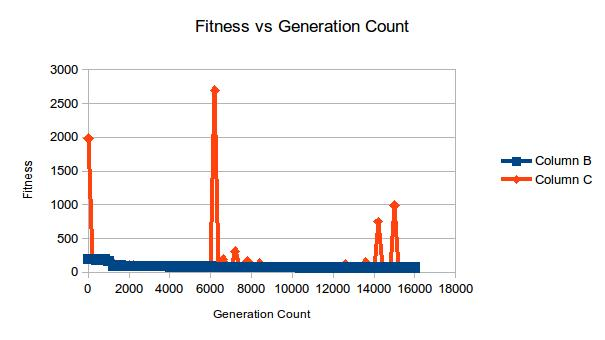
\includegraphics[width=.9\linewidth]{./fitness.jpg}
\caption{Average and best fitness for the symbolic problem. Best fitness has the perfect trend, but average fitness has several peaks due to the offspring outliers resulted from parent crossover and node mutation.}
\end{figure}
Figure 1 indicates that the crossover and node mutation works pretty well in that aspect that the best individual fitness from the population reduced down smoothly. 
From the above figure 1 we can also see that the average fitness has several peaks, that was due to the offspring outliers when two parent from previous generation crossover and node mutated. If I apply some tricks to filter out these outliers, and then calculate the population average, it should be able to get smoothly down average fitness as well.
\subsection{Applying best function on test points}
\label{sec-2-2}
\begin{figure}[htb]
\centering
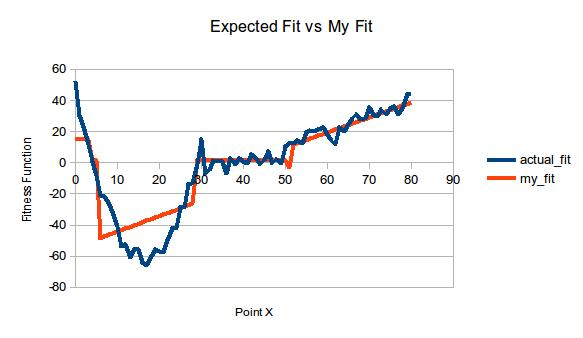
\includegraphics[width=.9\linewidth]{./fit3.jpg}
\caption{Expected fit and my fitness function. It seems like my fitness function still have some distance away from the expected fitness. One possible reason results this is that my crossover swap function almost do only non-terminal to non-terminal swap, terminal to terminal swap. But if I allow non-terminal to terminal swap, or terminal to non-terminal swap, it should have better results.}
\end{figure}
As can be seen from Figuare 2, it is a working algorithm, or in other words, code set, but still it has some ditance away from the expected one. Recall the algorithm that I have used, it was the crossover step that I have restricted the crossover node too restricted. Except the 90/10 non-terminal terminal rule, I have also restricted the crossover to be non-terminal to non-terminal swap, or terminal to terminal swap, but I should have allow non-terminal to terminal or terminal to non-terminal as well. 
\section{Conclusions}
\label{sec-3}
In order be able to do genetic programming, we need certain data structures that would allow us be able to swap the evoluationary algorithms data in the middle functionally as if we have swapped programs. Like this project, we used the tree structure. As far as we understand the Genetic Programming theory and C++ pointer, the project turned out to be not that hard. And so far, it works pretty well. 

But still, as can be easily seen from figure 2, there are quite some distance from the expected solutions. With deeper consideration of good-bad codes side-effects, and individual expression tree size control, hopefully by Project 2, I would be able to get better results that fits better and have limited bad codes in my best fit expression tree. 

\section{example results I got before bad$_{\text{alloc}}$}
\label{sec-4}
\begin{lstlisting}[language=c++]
jenny@jenny-G50VT ~/docu/572/b $ a
Population Information: 
min:198.373
avg:223771
avgSize:6.09
0        198.373         62508.3         6.15
10000    47.792          52.2099         228.71
20000    43.2229         47.4843         170.03
30000    40.6869         44.7676         178.67
40000    39.5117         40.8662         180.05
50000    39.1358         41.5992         186.31
60000    39.0548         41.1758         183
70000    39.013          44.1686         183
80000    38.7218         39.3482         183.3
90000    37.7194         40.3539         179.78
100000   36.9666         1945.47         188.16
110000   36.5285         38.7527         203.68
120000   36.3764         100.678         201.6
130000   36.3343         40.3855         199
140000   36.3302         56.5278         199
150000   36.3227         38.3612         199.15
160000   36.2536         60.347          204
170000   36.1636         40.8178         203.05
180000   36.1345         40.0999         203
190000   36.0784         41.1022         203.3
200000   35.9286         39.7798         206.87
terminate called after throwing an instance of 'std::bad_alloc'
  what():  std::bad_alloc
Aborted
jenny@jenny-G50VT ~/docu/572/b $ 
\end{lstlisting}
\section{A expression tree I have got}
\label{sec-5}
This fitness function is used for the test points plot, because this is the best tree that I have been able to save the expression tree results. Previous ones, like some function fitness can reach down to 35.9268, but I lost tract of the individuals when I got bad$_{\text{alloc}}$. 
\begin{lstlisting}[language=c++]
popu[9]:  Size: 43 Fitness: 102.65
F  
        +  
                X  
                3.40501  
        +  
                2.88043  
                11.9524  
        F  
                *  
                        X  
                        0.963943  
                F  
                        +  
                                X  
                                12.8615  
                        /  
                                7.2073  
                                5.11281  
                        *  
                                7.2073  
                                -4.63379  
                        /  
                                7.2073  
                                0.717242  
                F  
                        +  
                                X  
                                3.40501  
                        *  
                                7.2073  
                                -4.63379  
                        +  
                                2.88043  
                                11.9524  
                        /  
                                7.2073  
                                5.11281  
                -  
                        X  
                        14.3528  
        *  
                X  
                0.963943  
\end{lstlisting}
% Emacs 24.3.50.1 (Org mode 8.2.5h)
\end{document}